\documentclass[11pt,preprint, authoryear]{elsarticle}

\usepackage{lmodern}
%%%% My spacing
\usepackage{setspace}
\setstretch{1.2}
\DeclareMathSizes{12}{14}{10}{10}

% Wrap around which gives all figures included the [H] command, or places it "here". This can be tedious to code in Rmarkdown.
\usepackage{float}
\let\origfigure\figure
\let\endorigfigure\endfigure
\renewenvironment{figure}[1][2] {
    \expandafter\origfigure\expandafter[H]
} {
    \endorigfigure
}

\let\origtable\table
\let\endorigtable\endtable
\renewenvironment{table}[1][2] {
    \expandafter\origtable\expandafter[H]
} {
    \endorigtable
}


\usepackage{ifxetex,ifluatex}
\usepackage{fixltx2e} % provides \textsubscript
\ifnum 0\ifxetex 1\fi\ifluatex 1\fi=0 % if pdftex
  \usepackage[T1]{fontenc}
  \usepackage[utf8]{inputenc}
\else % if luatex or xelatex
  \ifxetex
    \usepackage{mathspec}
    \usepackage{xltxtra,xunicode}
  \else
    \usepackage{fontspec}
  \fi
  \defaultfontfeatures{Mapping=tex-text,Scale=MatchLowercase}
  \newcommand{\euro}{€}
\fi

\usepackage{amssymb, amsmath, amsthm, amsfonts}

\def\bibsection{\section*{References}} %%% Make "References" appear before bibliography


\usepackage[round]{natbib}
\bibliographystyle{plainnat}

\usepackage{longtable}
\usepackage[margin=2.3cm,bottom=2cm,top=2.5cm, includefoot]{geometry}
\usepackage{fancyhdr}
\usepackage[bottom, hang, flushmargin]{footmisc}
\usepackage{graphicx}
\numberwithin{equation}{section}
\numberwithin{figure}{section}
\numberwithin{table}{section}
\setlength{\parindent}{0cm}
\setlength{\parskip}{1.3ex plus 0.5ex minus 0.3ex}
\usepackage{textcomp}
\renewcommand{\headrulewidth}{0.2pt}
\renewcommand{\footrulewidth}{0.3pt}

\usepackage{array}
\newcolumntype{x}[1]{>{\centering\arraybackslash\hspace{0pt}}p{#1}}

%%%%  Remove the "preprint submitted to" part. Don't worry about this either, it just looks better without it:
\journal{Journal of Finance}

 \def\tightlist{} % This allows for subbullets!

\usepackage{hyperref}
\hypersetup{breaklinks=true,
            bookmarks=true,
            colorlinks=true,
            citecolor=blue,
            urlcolor=blue,
            linkcolor=blue,
            pdfborder={0 0 0}}


% The following packages allow huxtable to work:
\usepackage{siunitx}
\usepackage{multirow}
\usepackage{hhline}
\usepackage{calc}
\usepackage{tabularx}
\usepackage{booktabs}
\usepackage{caption}
\usepackage{colortbl}

\urlstyle{same}  % don't use monospace font for urls
\setlength{\parindent}{0pt}
\setlength{\parskip}{6pt plus 2pt minus 1pt}
\setlength{\emergencystretch}{3em}  % prevent overfull lines
\setcounter{secnumdepth}{5}

%%% Use protect on footnotes to avoid problems with footnotes in titles
\let\rmarkdownfootnote\footnote%
\def\footnote{\protect\rmarkdownfootnote}
\IfFileExists{upquote.sty}{\usepackage{upquote}}{}

%%% Include extra packages specified by user
% Insert custom packages here as follows
% \usepackage{tikz}

%%% Hard setting column skips for reports - this ensures greater consistency and control over the length settings in the document.
%% page layout
%% paragraphs
\setlength{\baselineskip}{12pt plus 0pt minus 0pt}
\setlength{\parskip}{12pt plus 0pt minus 0pt}
\setlength{\parindent}{0pt plus 0pt minus 0pt}
%% floats
\setlength{\floatsep}{12pt plus 0 pt minus 0pt}
\setlength{\textfloatsep}{20pt plus 0pt minus 0pt}
\setlength{\intextsep}{14pt plus 0pt minus 0pt}
\setlength{\dbltextfloatsep}{20pt plus 0pt minus 0pt}
\setlength{\dblfloatsep}{14pt plus 0pt minus 0pt}
%% maths
\setlength{\abovedisplayskip}{12pt plus 0pt minus 0pt}
\setlength{\belowdisplayskip}{12pt plus 0pt minus 0pt}
%% lists
\setlength{\topsep}{10pt plus 0pt minus 0pt}
\setlength{\partopsep}{3pt plus 0pt minus 0pt}
\setlength{\itemsep}{5pt plus 0pt minus 0pt}
\setlength{\labelsep}{8mm plus 0mm minus 0mm}
\setlength{\parsep}{\the\parskip}
\setlength{\listparindent}{\the\parindent}
%% verbatim
\setlength{\fboxsep}{5pt plus 0pt minus 0pt}



\begin{document}

\begin{frontmatter}  %

\title{A Data Scientific Approach to Equity Backtesting}

% Set to FALSE if wanting to remove title (for submission)




\author[Add1]{Riaz Arbi}
\ead{}





\address[Add1]{University of Cape Town, South Africa}


\begin{abstract}
\small{
Abstract to be written here. The abstract should not be too long and
should provide the reader with a good understanding what you are writing
about. Academic papers are not like novels where you keep the reader in
suspense. To be effective in getting others to read your paper, be as
open and concise about your findings here as possible. Ideally, upon
reading your abstract, the reader should feel he / she must read your
paper in entirety.
}
\end{abstract}

\vspace{1cm}

\begin{keyword}
\footnotesize{
Equity Backtesting \sep Reproducible Research \sep Event-based
Backtesting \sep R \sep RStudio \\ \vspace{0.3cm}
\textit{JEL classification} 
}
\end{keyword}
\vspace{0.5cm}
\end{frontmatter}


\renewcommand{\contentsname}{Table of Contents}
{\tableofcontents}

%________________________
% Header and Footers
%%%%%%%%%%%%%%%%%%%%%%%%%%%%%%%%%
\pagestyle{fancy}
\chead{}
\rhead{}
\lfoot{}
\rfoot{\footnotesize Page \thepage\\}
\lhead{}
%\rfoot{\footnotesize Page \thepage\ } % "e.g. Page 2"
\cfoot{}

%\setlength\headheight{30pt}
%%%%%%%%%%%%%%%%%%%%%%%%%%%%%%%%%
%________________________

\headsep 35pt % So that header does not go over title




\pagebreak

\section{\texorpdfstring{Introduction
\label{Introduction}}{Introduction }}\label{introduction}

Intro intro intro

This paper is organised as follows. Section \ref{Backtest section}
briefly introduces the practice of backtesting of investment strategies
in academia and industry, enumerates common methodological issues that
compromise the validity of research and discusses the replication crisis
that exists in both domains. Section \ref{Reproducible Research}
describes the goals and philosophy of the reproducible research movement
and its links to the open source software movement, with a special focus
on the R statistical programming language, the Tidy approach to data
organization and the use of scripting to facilitate reprducibility and
transparency in scientific research. Section
\ref{Backtester Documentation} introduces a backtesting template that is
roughly compatible with the structure of a research compendium - that
is, a template which constitutes a basic minimum viable unit of
reproducible research.

\pagebreak

\section{\texorpdfstring{Backtesting in Academia and
Industry\label{Backtest section}}{Backtesting in Academia and Industry}}\label{backtesting-in-academia-and-industry}

Investigations into why some stocks outperform others have a long
history. Professional bodies of knowledge, often captured in heuristics
or rules of thumb, have existed since at least the early 20th century.
For instance Graham, Dodd, and Dodd
(\protect\hyperlink{ref-Graham1934a}{1934}) released the first edition
of their \emph{Security Analysis} textbook in 1934. As time has
progressed, professionals and academics have sought to test these rules
in a rigorous manner, and to implement automated trading strategies
based on those rules that stand up to scrutiny.

Academics often frame this challenge as attempting to identify whether a
population subsetted by the presence or absence of an attribute exhibit
statistically significant differences in returns. Fama and French
(\protect\hyperlink{ref-Fama1992}{1992}), for instance, split the US
stock universe by market capitalization and market \(\beta\), and then
regress the cohorts against size, book to market, leverage and earnings
yield to investigate whether any of these variables have explanatory
power for outsize returns.

Traders, in contrast, tend to frame the question in terms of raw
performance - does a trading rule result in abnormal (risk adjusted)
returns over and above some benchmark? There is a rich ecosystem of
software packages, tutorials, online communities, books and blog posts
that attmepts to tackle this question (see Quantpedia
(\protect\hyperlink{ref-Quantpedia2018}{2018}) for a list of software
packages).

Confusingly, both of these broad approaches are encompassed by the
generic term `backtesting'. To avoid confusion, we adopt a broad
definition from D. H. Bailey et al.
(\protect\hyperlink{ref-Bailey2014}{2014}) :

\begin{quote}
A \emph{backtest} is a historical simulation of an algorthmic investment
strategy.
\end{quote}

Because these two communities frame the problem differently, they have
developed distinctive approaches. Academics tend to focus on using
statistical techniques to explain abnormal returns in terms of
independent variables. Traders tend to focus on prediction; trading
rules range from being extremely simple, such as moving averages, to
exceedingly complex implementations that use machine learning to
automatically select features (Peterson
(\protect\hyperlink{ref-Peterson2017}{2017})).

\subsection{Common areas}\label{common-areas}

A common area, however, is in interrogation. Both groups are concerned
with whether their result is robust. For both groups, a well-designed
backtest should yield results out of sample (OOS) which are similar to
results derived in sample (IS). Unfortunately, backtesting is a very
difficult operation to achieve correctly, and as a result it is quite
easy to derive rules which perform well IS but poorly OOS (D. H. Bailey
et al. (\protect\hyperlink{ref-Bailey2014}{2014})).

Because of this common concern, there common opinion on how to
appropriately construct datasets and to assess whether a result is
robust.

\subsubsection{\texorpdfstring{Data quality
issues\label{Data Quality}}{Data quality issues}}\label{data-quality-issues}

Every backtest needs a historical dataset upon which to simulate a
trading strategy. This dataset needs, at a minimum, to contain a time
series of every member of the stock universe with price returns and any
other attributes that may serve as inputs to the trading rule. This
minimal dataset is necessary, but not sufficient, for a realistic
backtest.

A realistic backtest also needs to address the following data quality
issues:

\begin{enumerate}
\def\labelenumi{\arabic{enumi})}
\item
  Does the dataset contain \emph{survivorship bias}? At present,
  constituents of a stock universe are survivors. They are, by
  definition, the stocks which have not disappeared from the universe
  because of bankruptcy, delisting or mergers. To base our data only on
  this group will mean that we apply the rule only to a very particular
  subset of a stock universe: those destined to remain listed. Since
  this implicit filter cannot be applied going forward (i.e we cannot
  filter our existing unuverse to include only those that will be listed
  at some arbitrary point in the future), our IS result is likely to be
  different from our OOS result.
\item
  Does the dataset contain \emph{look-ahead bias}? There are many ways
  that we can implicitly `peek' into the future with histrical datasets.
  A common pitfall is to use the `close' price as representative of a
  day's average price. This, of course, uses future data because the
  close price cannot be known before the end of day. Another example is
  the inappropriate joining of fundamental and market data. Fundamental
  data is usually timestamped to the time at which the fact was true in
  the real world. However, these facts only become known at a (typically
  much later) future date. The Currenr Assets at 31 December 2003, for
  instance, is only known at release of the annual financial statements,
  which might have been on the 27th February 2004. Joining this data
  point to marke tdata on the date 31 December 2003 will introduce
  look-ahead bias to your dataset.
\item
  Is the dataset \emph{complete}? Some datasets contain more information
  than others. Trice (\protect\hyperlink{ref-Trice2017}{2017}) compares
  data for the S\&P 500 Index across the free data vendors Google.com
  and Yahoo.com and finds discrepancies between them - the salient chart
  is reproduced below. In this instance, the discrepancy derives from
  the fact that Google contains a significant number of N/A values,
  which skew the summary statistics.
\end{enumerate}

\begin{figure}
\centering
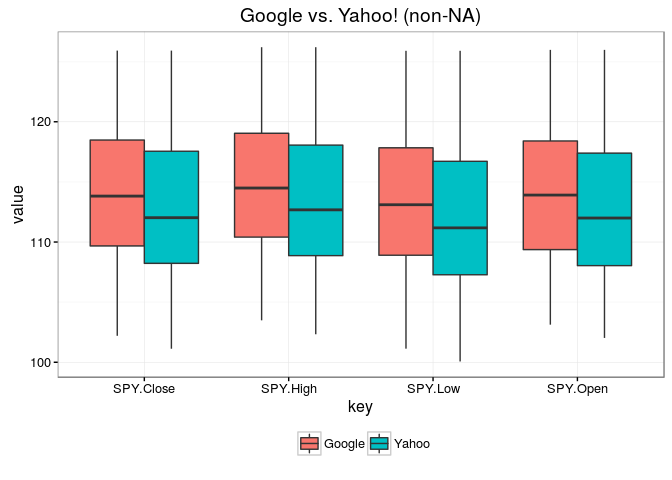
\includegraphics{/home/riaz/projects/equity_analysis/paper/source/data/data-quality-a-boxplot-1.png}
\caption{Data Discrepancies between Google and Yahoo! (Trice
(\protect\hyperlink{ref-Trice2017}{2017}))\label{Table1}}
\end{figure}

\begin{enumerate}
\def\labelenumi{\arabic{enumi})}
\setcounter{enumi}{3}
\tightlist
\item
  Does the dataset contain \emph{retroactive corrections}? It is common
  for companies to restate financial information after the fact. This
  can be because of changes in accountng rules, new information that
  comes to light, or to aid in comparison across major changes to the
  company structure. If these restatements are retroactively applied to
  a dataset, they can introduce look-ahead bias.
\end{enumerate}

\subsubsection{Modeling issues}\label{modeling-issues}

Regardless of the backtest approach, the following issues need to be
taken into account to assess the realism of the model:

\begin{enumerate}
\def\labelenumi{\arabic{enumi})}
\item
  Has \emph{market impact} been taken into account? Return anomalies may
  appear to exist be related to illiquidity. That is to say, the returns
  of a stock (or class of stocks) may appear to be abnormal, but the
  abnormal returns may be due to the market impact of a trade on the
  stock. A realistic model will adjust for this by assuming minimal
  impact for only a small fraction of daily volume traded, build in a
  price impact if the trade size exceeds this volume, and respect the
  bid/ask spread when desiding that a trade matches.
\item
  Have \emph{transaction costs} been taken into account? Similar to
  market impact, transaction costs form varying percentages of a trade;
  this depends on the commission structure. A class of stocks may appear
  to exhibit abnormal returns but all suffer from high transaction costs
  because they are, for instance, penny stocks that all require an
  exhorbitant minimum commission for small lots.
\item
  Failing to account for \emph{short positions or portfolio bankruptcy}.
  Portfolios can be long only or allow for short positions. Short
  positions involve interest charges that need to be taken into account.
  Long only portfolios cannot have negative positions. Similarly,
  portfolio cash balances cannot be negative of no leverage (which
  attract interest charges) is employed. Portfolio bankruptcy needs to
  be accounted for - if a strategy has an average excess return of 2\%,
  but there are two periods in which the return is -100\%, then the
  average return does not matter.
\item
  Data mining and \emph{backtest overfitting}. When a researcher
  iterates over many strategies while recycling the same dataset, is is
  easy to overfit a model. Overfitting a model is when one selects rules
  which perform well in sample but poorly out of sample. That is, they
  model the noise in the training set, not the signal (D. H. Bailey et
  al. (\protect\hyperlink{ref-Bailey2014}{2014})). This possibility is
  especially acute in the age of hyperparameter tuning and feature
  selection, where a computer can modify large numbers of parameters at
  once to select ones that perform optimally. This can be delat with by
  keeping track of the number of trials and adjusting the hurdle for
  statistical significance accordingly, or testing for path-dependency,
  which is an indicator that a model has been tuned for a particular
  path-dependent series, as opposed to an underlying signal (Lopez de
  Prado (\protect\hyperlink{ref-LopezdePrado2013}{2013})).
\end{enumerate}

\subsection{The Replication Crisis}\label{the-replication-crisis}

While total data fidelity and perfect model specification are good goals
in theory, the reality is that compromises often need to be made. It is
often simply impossible to model the exact market impact a trade will
have; data may not be avaialable at sufficient detail; information on
when fundamental data was released may simply not exist.

Inevitably, a researcher needs to make judgment calls. A typical
backtest involves many judgment calls; these permeate the entire
analysis chain from deciding what source data to use all the way through
to deciding which metrics to use to evaluate strategy success.

\subsubsection{In academia}\label{in-academia}

It is a standard aspiration for researchers to disclose all the judgment
calls made during the backtest process, but these disclosures are
invariably incomplete. This makes validation by other researchers very
difficult. At the extreme, independent validators may arrive at a
completely different conclusion (Hou, Xue, and Zhang
(\protect\hyperlink{ref-Hou2017}{2017})); with ambiguity on both sides
it is unclear whether the discrepancy is due to differences in
underlying data, prepearation methodologies, mathematical errors or some
other factor unrelated to the question at hand.

The academic discipline of anomalies research has grown into a
substantial corpus of contradictory claims. These contradictions are
mirrored in the business of investment management by competing
investment philosopies, each with its own library of peer-reviewed
papers (Damodaran (\protect\hyperlink{ref-Damodaran2012}{2012})). While
markets may very well accommodate contradictory drivers of returns it is
often difficult to discern whether differing claims are the result of
geniune facts or the result of methodological differences.

Hou, Xue, and Zhang (\protect\hyperlink{ref-Hou2017}{2017}) attempt to
replicate the entire anomalies literature to identify with results can
actually be confirmed. They attempt to replicate 447 anomalies and find
that between 64\% and 85\% of them are insignificant. In other words,
they suspect widespread misuse of statistical analysis to make claims
that are not, in fact, true. This is possible, in part, because
practitioners have a large degree of discretion in determining every
aspect of the backtesting analysis chain. Hou, Xue, and Zhang
(\protect\hyperlink{ref-Hou2017}{2017}) attempt to set out a common set
of replication procedures to standardise research output, including (but
not limited to):

\begin{itemize}
\tightlist
\item
  Specifying datasets: Compustat Annual and Quarterly Fundamental Files;
  Center for Research and Security Prices (CRSP).
\item
  Specifying breakpoints: Use NYSE breakpoints
\item
  Use value-weighted, not equal-weighted portfolios
\item
  No sample screening (ie don't exclude stocks because of some arbitrary
  cutoff)
\item
  For annually-composed portfolios, resort at the end of June
\item
  Incorporate fundamental data four months after valid date
\end{itemize}

Many of the above guidelines are designed to avoid outsize effects from
micro capitalization shares, which form 3\% of market value but comprise
60\% of the total number of stocks. These stocks often suffer from high
transaction costs and low liquidity, which muddy the waters when testing
for a particular factor.

\subsubsection{In industry}\label{in-industry}

Unfortunately, these guidelines are not directly applicable to
backtesting for trading. Traders are primarily interested in real-world
excess returns; the use of CRSP prices to compute returns, for instance,
does not translate into real cash balances.

The approach taken by developers of trading backtesters has been to
build engines which are capable of easily switching between simulated
and real-life trading. The rationale is that, as long as the data is
from the same source, signal generation, trade matching, transaction
costs, account balances and portfolio composition can operate
unmodified. This somewhat mitigates concerns around replicability - if
it works on historical data, simply switch the data source to live data
and don't ask too many questions.

The caveats are as follows. Firstly, many of these engines are
proprietary (Quantpedia (\protect\hyperlink{ref-Quantpedia2018}{2018}))
and the actual mathematics of what is going on is not available, which
means that the researcher has to take it on faith that the
implementation (and source data) is correct. If IS results differ from
OOS results it is difficult to debug where the issue is: it could be
data quality, poor implementation, or overfitting. One cannot be certain
that one's returns are being driven by the reasons one thinks.

There do exist many open source backtesting libraries, most notably the
\texttt{zipline} python package (Zipline
(\protect\hyperlink{ref-Zipline2018}{2018})), the Quantopian trading
platform (Quantopian (\protect\hyperlink{ref-Quantopian2018}{2018})),
which is built on top of \texttt{zipline}, and the R package
\texttt{quantstrat} (Carl et al.
(\protect\hyperlink{ref-Carl2018}{2018})).

Although these packages make it possible to inspect the entire
analytical chain they do not provide historical data. Historical data is
difficult (and expensive) to procure, and the same concerns raised in
\ref{Data Quality} still exist. In many ways, these issues are worse
because these packages default to free data sources such as Yahoo!,
Google Finance or Quandl, which do not document index constituent
membership changes, retroactive data modification or provide any
guarantees of veracity. Bias-free data must be procured, cleaned and put
in an appropriate format beforehand; documentation of how to conduct
these operations is left as an exercise to the researcher. Even if a
researcher can procure well-formed, comprehensive data, there exists no
toolset to transform that data into an appropriate format for ingestion
to any particular software package, and no tools to investigate the
health of the data with reference to the biases mentioned in
\ref{Data Quality}.

These shortcomings in free data sources drive areas of research: the
documentation on \texttt{zipline}, Quantopian and \texttt{quantstrat}
focus overwhelmingly on price signals (algorithms relying on non-market
data such as fundamental, macroeconomic or alternative data are scarce)
and single-stock or fixed-basket portolios. This makes them much less
suitable for research into general strategies that can be applied across
an entire universe or research which relies on more than just market
data.

These backtesting packages are able to easily switch between simulated
and live trading because they implement event-based backtesting methods.
Event-based backtesting allow a trader to step through time, either in
fixed increments or through the consumption of a continuous information
stream, and trigger actions according the the information made available
to them. If implemented correctly, the event stream can be switched from
a historical dataset to a real-time stream with minimal changes to the
code. This eliminates a possible source of error: the algorithm does not
need to be rewritten into a live implementation.

There is something of an uncanny valley here. It is difficult for
industry practitioners to translate findings in anomalies research into
actionable strategies because of incomplete documentation and it is
difficult for academics to use production-level backtesters to search
for new anomalies. Part of this is because they have differing
objectives. But another hurdle is the steep learning curve required to
understand what is going on `under the hood' of a production trading
engine. Both \texttt{zipline} and \texttt{quantstrat} implement the
Object Oriented Programming (OOP) paradigm, which forces on objects
rather than procedures (Van Roy
(\protect\hyperlink{ref-VanRoy2009}{2009})). This is in contrast to a
Procedural approach, which focuses on operations (i.e taking an input,
performing an operation, and producing an output). OOP programs scale
well, and enable encapsulation: knowledge of the implementation of an
object is not necessary for its use. This provides convenience and
lowers barriers to entry for new users, but comes at a cost: linear
mapping of the sequence of procedures that constitute an operation can
be difficult.

Procedural programs, on the other hand, can typically be read from top
to bottom, and the procedural flow is often quite easy to follow.
Unfortunately, as the size of a program grows, the complexity and
brittleness of a procedural program increase super-linearly, as the
procedure has to incorporate more and more subroutines to manage the
various inputs and outputs of a particular part of the program.

\pagebreak

\section{\texorpdfstring{Reproducible Research and The R Programming
Language\label{Reproducible Research}}{Reproducible Research and The R Programming Language}}\label{reproducible-research-and-the-r-programming-language}

Problems with replication are not unique to backtesting. Science, as a
whole, is experiencing a replication crisis.

Despite scientific research being an accretive process, involving
verification and building upon earlier datasets and findings, the
computational work done by researchers is often poorly documented, or
absent (Stodden et al. (\protect\hyperlink{ref-Stodden2013}{2013})).
This introduces the risk that views or principles that are considered to
be scientifically verified may, in fact, be false.

Gaps in documentation allow bad reasoning, calculation errors or
spurious results to creep in to the corpus of knowledge of a discipline
because peers are forced to take it on faith that a researcher has a
proper understanding of underlying mathematical concepts, and that
workings have been thouroughly cross-checked before release.

Worse still, because follow-up replication is difficult to impossible
with poor documentation or data availability, incorrect beliefs can
persist for years, or even decades (Munafò et al.
(\protect\hyperlink{ref-Munafo2017}{2017})). \emph{P-hacking}, or the
selection of data and finessing of results to conform to significance
tests of 5\% or lower, has resulted in a situation where a research
finding is as likely to to be false it is to be true (J. P. A. Ioannidis
(\protect\hyperlink{ref-Ioannidis2005}{2005})).

Up until the late 20th century, practical constraints limited the amount
of supporting material a researcher could distribute along with a
research paper. Documentation of evey single mathematical operation
conducted with pencil and paper would be extremely laborous; duplication
and distribution of source data and computations would be extremely
expensive. However, in recent years, as computational power and storage
has become increasingly cheap and available, there have been persistent
calls for a review of the way that scientific research is packaged and
presented (Stodden et al. (\protect\hyperlink{ref-Stodden2013}{2013}),
Koenker and Zeileis (\protect\hyperlink{ref-Koenker2009}{2009})).

\subsection{Reproducible Research
Terminology}\label{reproducible-research-terminology}

In response to these calls, a taxonomy of reproducibility has emerged,
allowing peers to effectively categorize research.

This taxonomy allows us to dinstinguish reveiwability (which assumes
mathematical competence and focuses on reasoning) from reproducibility
(which allow the extension of the review into assessement of
mathematical competence and quality of data).

\begin{longtable}[]{@{}ll@{}}
\caption{Common Terminology in Reproducible Science (Stodden et al.
(\protect\hyperlink{ref-Stodden2013}{2013}))\label{Table1}}\tabularnewline
\toprule
\begin{minipage}[b]{0.18\columnwidth}\raggedright\strut
Term\strut
\end{minipage} & \begin{minipage}[b]{0.61\columnwidth}\raggedright\strut
Description\strut
\end{minipage}\tabularnewline
\midrule
\endfirsthead
\toprule
\begin{minipage}[b]{0.18\columnwidth}\raggedright\strut
Term\strut
\end{minipage} & \begin{minipage}[b]{0.61\columnwidth}\raggedright\strut
Description\strut
\end{minipage}\tabularnewline
\midrule
\endhead
\begin{minipage}[t]{0.18\columnwidth}\raggedright\strut
Confirmable\strut
\end{minipage} & \begin{minipage}[t]{0.61\columnwidth}\raggedright\strut
Main conclusions can be attained independently\strut
\end{minipage}\tabularnewline
\begin{minipage}[t]{0.18\columnwidth}\raggedright\strut
Reviewable\strut
\end{minipage} & \begin{minipage}[t]{0.61\columnwidth}\raggedright\strut
Descriptions of methods can be independently assessed and judged\strut
\end{minipage}\tabularnewline
\begin{minipage}[t]{0.18\columnwidth}\raggedright\strut
Replicable\strut
\end{minipage} & \begin{minipage}[t]{0.61\columnwidth}\raggedright\strut
Tools are made available that would allow duplication of results\strut
\end{minipage}\tabularnewline
\begin{minipage}[t]{0.18\columnwidth}\raggedright\strut
Auditable\strut
\end{minipage} & \begin{minipage}[t]{0.61\columnwidth}\raggedright\strut
Sufficient records exist (perhaps privately) to defend research\strut
\end{minipage}\tabularnewline
\begin{minipage}[t]{0.18\columnwidth}\raggedright\strut
Reproducable\strut
\end{minipage} & \begin{minipage}[t]{0.61\columnwidth}\raggedright\strut
Auditable research is made openly available, including code and
data\strut
\end{minipage}\tabularnewline
\begin{minipage}[t]{0.18\columnwidth}\raggedright\strut
To Verify\strut
\end{minipage} & \begin{minipage}[t]{0.61\columnwidth}\raggedright\strut
To check that computer code correctly performs the intended
operation\strut
\end{minipage}\tabularnewline
\begin{minipage}[t]{0.18\columnwidth}\raggedright\strut
To Validate\strut
\end{minipage} & \begin{minipage}[t]{0.61\columnwidth}\raggedright\strut
To check that the results of a computation agree with observations\strut
\end{minipage}\tabularnewline
\bottomrule
\end{longtable}

This paper uses reproducibility in the sense defined in \ref{Table1},
which is to say, it refers to research output being bundled and
distributed with well documented, fully transparent code and data that
allows a peer to fully review, replicate, audit and thereby confirm
results of a body of work (Stodden et al.
(\protect\hyperlink{ref-Stodden2013}{2013})).

\subsection{The Relationship between Reproducible Research and Open
Source
Software}\label{the-relationship-between-reproducible-research-and-open-source-software}

Open source software development principles exhibit properties which are
useful to practitioners of reproducible research.

In general, software is written in text files, by humans, in a
particular programming language. This \emph{source code} is
\emph{compiled} or \emph{interpreted} by another program into binary
machine code (which is not readable by humans) and distributed for
execution. The software for the popular spreasheet program Microsoft
Excel, for instance, would be written by a group of humans in a
programming language. These text files would be compiled by a compiler
program into a binary executable program, which is distributed to
consumers who can execute the binary. When someone clicks the Excel icon
on their computer to `launch' the program, they are executing the
binary.

Open source software is software for which the \emph{source code} is
made publically available. Microsoft Excel is closed source, and the
source code is not made available. Source code can be read by humans,
binary cannot. Changes to source code can be meaningfully interpreted by
humans, because one can read the changes in plain text. Changes to
binary code cannot be interpreted by humans, because the changes are
simply alterations to a very long sequence of \texttt{0} and \texttt{1}
digits. It is trivial to compile source code into binary code. It is
extremely difficult to accurately decompile binary code into source
code, and the tools are not readilty available (Li
(\protect\hyperlink{ref-Li2004}{2004})).

By definition, the text-based nature of source code makes all source
code reproducible (and, by corollary, auditable). The implications of
this are twofold. Firstly, a researcher using open source software for
computation can be assured that the full software stack will be open to
scrutiny. That is, at the limit, an auditor could inspect every single
line of code from some arbitrary `open starting point' up to verify that
the computations are correct. This `open starting point' is as the
operating systme level for Linux based machines, and from the
application level up for Mac and Windows based machines.

Secondly, and perhaps more importantly, the open source software
community has decades of experience in defining good practices for
creating and maintaining large, open, verfiable and repeatable
enviroments. These principles are often quoted in the folkloric `Unix
Way', which manifests in epithets such as ``text is the universal
interface'' (Baum and Sirin (\protect\hyperlink{ref-Baum2002}{2002})),
``each unit should do one thing and do it well'', and ``build things to
talk to other things'' (Raymond
(\protect\hyperlink{ref-Raymond:2003:AUP:829549}{2003})). Reproducible
research practice is built on the same principles - simple, readable
text-based data and code where possible; clear separation between data,
code and results; complete transparency coverage; and portability by
design (see Baum and Sirin (\protect\hyperlink{ref-Baum2002}{2002}),
Bache and Wickham (\protect\hyperlink{ref-Bache2014}{2014}), Wickham
(\protect\hyperlink{ref-Wickham2014}{2014})).

Historically, there has been close collaboration between the open source
software and the free software communities. This means that, as a rule,
most open source software is free or has a free analogue. The core tools
of Data Science, for instance (such as the python and R programming
languages, the Apache Foundation of big data processing packages and the
Jupyter and RStudio interactive development environemnts), are all open
source and free. This means that the \emph{cost} of replication is not
prohibitive: in general, reproducible research should be reproducible
for free on commodity hardware.

\subsection{The Suitability of R for Reproducible
Research}\label{the-suitability-of-r-for-reproducible-research}

The R programming language was originally conceived as a project to
build out an open source statistical programming environment. In
development since 1997, base R is now a mature ecosystem comprising a
scriptable language, graphical rendering system and debugger (R Core
Team (\protect\hyperlink{ref-RCoreTeam2018}{2018})). A large community
of third party developers (some commercial, most free) have extended
base R with over 13000 packages, including a fully-fledged interactive
development environmnent (Rstudio), interactive dashboarding web server
(Shiny) and bindings to LaTex for simple rendering of publication-ready
LaTex documents from markdown (knitr and rmarkdown) (RStudio Team
(\protect\hyperlink{ref-RStudioTeam2015}{2015})). Because of its roots
in open source, it adheres to many open source software conventions. For
instance-

\begin{itemize}
\tightlist
\item
  All source code is freely available
\item
  All development work in R is done in plain text files, which are
  transparently human and machine readable.
\item
  The R project has adopted the GNU General Public License verison 2,
  which ``does not restrict anyone from making use of the program in a
  specific field of endeavor'' (R Core Team
  (\protect\hyperlink{ref-RCoreTeam2018}{2018})). This free
  avaialability means that anybody with a commodity computer and an
  internet connection can install and use R.
\end{itemize}

Although the reproducible research community is principles-based and
language-agnostic, the free, text-based nature of the R language have
made it a good candidate for reproducible work (Gentleman and Lang
(\protect\hyperlink{ref-Gentleman2004}{2004})). Marwick, Boettiger, and
Mullen (\protect\hyperlink{ref-Marwick2018}{2018}) review the concept of
a \emph{research compendium}, and explore how research done in R can be
packaged into compendia. They argue that a compendium is defined by
three principles -

\begin{enumerate}
\def\labelenumi{\arabic{enumi}.}
\tightlist
\item
  Files should be organised according to a prevailing standard so that
  others can immediately understand the structure of the project, and
  pipe the compendium to environments that expect the standard structure
  with no structural modifications.
\item
  Maintain a clear separation between data, method and output.
  Separation means that data is treated as read only, and that all steps
  in getting from source data to output is documented. Output should be
  treated as disposable, and rebuildable from the programmatic
  application of the method to the data.
\item
  Specify the computational environment that was used to conduct the
  research. This provides critical information to a replicator on the
  undelrying tooling needed to support the analysis.
\end{enumerate}

These principles are intended to ensure that, given a certain input (the
data) and a certain operation (the method), a deterministic output
results (the analysis). With these details out of the way, an auditor
can focus on verifying the correctness of the reasoning (i.e should we
use this theory) and of the implementation (i.e are there any errors in
the math).

The richness of the R ecosystem means that one can complete the full
research life cycle from data loading to publishing without leaving the
R ecosystem (Baumer et al. (\protect\hyperlink{ref-Baumer2014}{2014})).
Data can be loaded, cleaned, transformed, modeled and aggregated in R.
The results can be written up in RStudio - in fact, the code and
write-up can be combined into a single text-only document using the
RMarkdown format - and exported to a wide range of academically accepted
typsets and formats (such as Tex, Microsoft Word, Markdown and HTML).
Because R is scriptable, R scripts can also be used in production
environments, where results can be periodically recomputed and handed on
to some other production process.

This property dramatically simplifies the complexity of building a
compendium and the required skill-set of a replicator. For instance, a
single-platform research compendium can be assessed by anyone with
knowledge of that single environment. Multi-platform compendia need
replicators well-versed in each platform, which dramatically reduces the
pool of potential replicators.

Upon publication, code versioning tools such as Git allow the public to
view all future changes to the code or data transparently, and, if code
changes over time, to assess the impact of those changes on the result.

\subsection{Tidy Extensions to Base R}\label{tidy-extensions-to-base-r}

The open source and reproducible science principles of interoperability,
readibility, modular code and common standards have been extended into
the prcatice of data manipulation by Wickham
(\protect\hyperlink{ref-Wickham2014}{2014}). The collection of R
packages which fall under this banner are collectively known as the
`Tidyverse'. These packages provide a common, idiosyncratic syntax for
data ingestion, munging, manipulation and visualization that are
opinionated in their expectations about data structure and focused on
enabling readable code (Wickham
(\protect\hyperlink{ref-Wickham2017}{2017})). According to Wickham, tidy
data intuitively maps the meaning of a dataset to its structure -

\begin{quote}
\begin{enumerate}
\def\labelenumi{\arabic{enumi}.}
\tightlist
\item
  Each variable forms a column.
\item
  Each observation forms a row.
\item
  Each type of observational unit forms a table.
\end{enumerate}
\end{quote}

Whether there is a single optimal data structure is up for debate. What
is not up for debate is that that the adoption of a common standard for
structures allows researchers to make assumptions about the meaning of
data before engaging with the content, i.e simply knowing that data is
`tidy' means that a researcher knows that each column maps to a
variable, and each row an observation, \emph{prior to looking at the
data}. Setting of standards enables the decoupling of processes -
process (a) can produce some peice of analytical output \emph{with no
knowledge of what it will be used for}. As long as it is `tidy', and
process can consume that output on the understanding that is confirms to
the `tidy' standard and take the analysis further. In this way, the
`tidy data' concept push the Unix Way concept of `build things that talk
to other things' into the practice of structuring data for reproducible
research.

\subsection{The Potential for Reproducible Research to Address The
Replication Crisis in Anomalies
Research}\label{the-potential-for-reproducible-research-to-address-the-replication-crisis-in-anomalies-research}

We have explored how the sheer number of judgment calls involved in
building a rigorous backtest inhibit replicability, both in academia and
in a prefessional setting. Obstacles differ between them; academics
suffer from incomplete documentation, professional traders suffer from a
dearth of simple, transparent toolkits to automate the entire analysis
chain. Both communities have serious shortcomings when it comes to
transparent data acquisition and preparation.

We have also shown how these obstacles are being addressed in the
scientific community at large by the concepts of reproducible research,
the research compendium and Tidy Data. These concepts are supported by
certain technologies: cheap commodity computing, free and open source
scientific computing software and text versioning tools in general, and
the R programming language and ecosystem for acquisition-to-publication
analysis in particular.

It stands to reason that the concepts and tools of reproducible research
could be used to address the issues in backtesing at large. These tools
would have to -

\begin{enumerate}
\def\labelenumi{\arabic{enumi}.}
\setcounter{enumi}{3}
\tightlist
\item
  Be able to run on a typical researcher's computer
\item
  Produce artifacts (models and data objects) that are portable across
  the academia / industry divide
\item
  Encompass the full analysis chain from aquisition through to
  reporting, with a particular focus on raw data processing
\item
  Accommodate deep customizability without requiring excessive
  complexity of code
\item
  Expose underlying workings in a transparent, procedural manner to an
  auditor
\end{enumerate}

It is crucial to bear in mind that the objective of such an
implementation would not be to build a rigorous backtest. Rather, its
immediate goal would be to build a totally transparent engine that
places ease of audit first and foremost. Borrowing a concept from the
open source community, it is assumed that stability and correctness of
implementation are derivative properties of a rigorous, continuous
review process.

These objectives are possible within the current capabilities of the R
ecosystem right now.

\begin{enumerate}
\def\labelenumi{\arabic{enumi}.}
\tightlist
\item
  R and all R packages run on any x86 processor
\item
  Research compendia are structured with portability in mind. The
  scripting capabilities of R allow an end-user to run the entire
  backtest non0-interactively if desired.
\item
  R, RStudio and the Tidyverse are a mature toolkit for end-to-end
  research
\item
  Like any programming language, R accommodates the creation of
  parameter variables which can be passed to user defined functions.
  These parameters can be altered in a transparent manner. Enhancements
  and additions to the engine code are completely trasparent and can be
  easily tracked with versioning tools such as git.
\item
  Although R has some OOP concepts, it is primarily a procedural
  language, which lends itself to a linear, top-to-bottom logical code
  flow
\end{enumerate}

In the following section we detail a rudimentary reference
implementation of a reproducible backtester.

\pagebreak

\section{\texorpdfstring{A Reference Implementation of a Data Scientific
Equity Backtester in
R\label{Backtester Documentation}}{A Reference Implementation of a Data Scientific Equity Backtester in R}}\label{a-reference-implementation-of-a-data-scientific-equity-backtester-in-r}

We provide an example of a reproducable equity backtesting workflow that
covers the full data processing chain from acquisition to reporting.

All code is available at
\url{http://github.com/riazarbi/equity_analysis}.

The data processing scripts can consume multiple data sources, for
multiple equity indexes, for any timeframe, for arbitrary data
attributes. The implementation is index-based. That is, data acquisition
begins with obtaining constituents for an equity index at a point in
time, and then proceeds to obtaining metadata and timeseries attributes
for the constituents.

Data queries are scripted, and therefore fully reproducible, and
repeatable. All queries are saved to a log directory. Reference datasets
are generated from the log directory. We use rudimendary log compaction
and data versioning to enable point-in-time analysis and check data
quality.

Datasets are read into memory for backtesting, which is done in a
step-through fashion. That is, the backtester steps through time, is
presented with data that would have been available to it at that date,
and executes trading rules which are persisted to a trade log and
trasnaction history.

This backtester has been built for multi-trial, parametrised backtesting
in mind. That is, certain global parameters are set (backtest start and
end date, target index etc) and then multiple user-specified algorithms
are tested at once. We adopt the multi-trial approach to facilitate
control for backtest overfitting, as per Lopez de Prado
(\protect\hyperlink{ref-LopezdePrado2013}{2013}).

We have built rudimentary support for transaction costs and slippage;
these can be extended in a transparent manner.

Input data has been segregated from results; it is anticipated that a
researcher will delete the input data prior to distribution to avoid
proprietary vendor licensing issues; this raw data should be regerated
from source using supplied query scripts.

\subsection{Intended Audience}\label{intended-audience}

This project should be useful to:

\begin{itemize}
\tightlist
\item
  Finance students at all levels wanting to conduct statistically
  rigorous equity backtests
\item
  Post graduates and academics looking to conduct research on a common
  platform to facilitate replication and peer review
\item
  Research professionals looking to build out an in-house backtesting
  environment for proprietary equity investment strategies
\item
  Equity researchers looking for a bridge between Excel-based research
  and \texttt{R} or \texttt{python}.
\end{itemize}

\subsection{Intended Use Case}\label{intended-use-case}

It is intended that a researcher will clone this repository to a local
directory and then create an RStudio project in the project root
directory. After querying data from an appropriate vendor and processing
the data using \texttt{scripts/1\_process\_data.R}, a researcher will
specify global parameters in the \texttt{scripts/run\_trials.R} file and
place a batch of algorithms in the \texttt{trials/} directory. Running
the \texttt{scripts/2\_run\_trials.R} script will backtest each
algorithm and save the results in the \texttt{results/} directory.
Running \texttt{scripts/3\_cross\_validate.R} will run the R package
\texttt{pbo} to test for the probability of backtest overfitting.

These results will be used to create a research paper, which can be
saved to the project root. Prior to release, the researcher can delete
the source data for licensing reasons (but retain the query scripts!)
and publish the entire compendium to a code hosting site such as
\href{https://github.com}{GitHub}.

\subsection{Included Data}\label{included-data}

This repository \textbf{does not include any equity data}, but it does
include working scripts to automatically extract data from data vendors,
and to save that data on a well-formed way. It is assumed that the user
will acquire data using the scripts which have been included in this
repository. This will only be possible if a user has access to the
relevant data services - namely Bloomberg, DataStream or iNet.

We also include a script for generating a range of simulated index
datasets, complete with constituent lists, metadata and market and
fundamental ticker timeseries. These datasets can be used to explore the
functioning of the code and test that it is working as expected.

\subsection{Future Development}\label{future-development}

This project is ongoing, and many rudimentary features will be refined
as time unfolds. For this reason, we recommend that users fork the
project prior to use, in order to lock their research to a particular
version of the compendium. Users are encouraged to submit pull requests
on \href{https://github.com}{GitHub} for bug fixes and to add features.

\subsection{Intellectual Property
Statement}\label{intellectual-property-statement}

This is the intellectual property of Riaz Arbi. This code will be
released under a strong copyleft license. A license is included in the
repository.

\newpage

\section{Detailed Documentation, With Design
Justifications}\label{detailed-documentation-with-design-justifications}

Because the workflow is linear and procedural in design, this
documentation will proceed in a linear, procedural fashion. After
familiarising the reader with the directory structure, we will work
through the code in a stepwise fashion from data acquisition through to
final reporting.

\subsection{Design Considerations}\label{design-considerations}

Because this compendium is designed to be run by researchers on
commodity consumer hardware, our design choices sacrifice speed in order
to keep memory usage low. We have split the backtesting procedure into
four stages - querying, data processing, backtesting, cross-validation
and reporting. Each stage expects to read in files from a pre-specified
location and writes files to a prespecified location. Often the first
script in a stage will clear the environment in order to release memory.

This has the added benefit of making these stages asynchronous.
Processing data does not require a new query to have been conducted;
cross validation does not require new trials to be run. These stages can
even be run on different machines that share network drives - although
the benefits will only be apparent if each stage's processing time is
longer than the network transfer time.

Where possible, we have made I/O optimizations. This includes converting
\texttt{.csv} files to \texttt{.feather} files, which are much faster to
read and write, and parallelizing select prices of code. Ticker-wise
data pipelining is multi-threaded, and the trading engine could be sped
up by making each trial run on its own thread.

All the actions required to conduct a complete backtest are captured in
plain text files. This means that every single computation and data
manipulation can be inspected and its functioning verified. The entire
code base can be versioned using a software verisoning tool such as git.
A researcher can fork this codebase, modify it, and push the
modifications back to the origin. All of these changes are immutably
recorded; future researchers can alway see exactly what has changed, who
has made the changes and what the reason for the change was.

\subsection{Directory Structure}\label{directory-structure}

The directory structure loosely conforms to Marwick, Boettiger, and
Mullen (\protect\hyperlink{ref-Marwick2018}{2018})'s definition of a
valid R packages structure, and most closely resembles the author's
example of an intermediate-level compendium. The root directory contains
the following files and directories:

\begin{itemize}
\tightlist
\item
  A \texttt{README.md} file that describes the overall project and where
  to get started.
\item
  A \texttt{Dockerfile} allows a user to build docker image identical to
  the researcher's environment.
\item
  A \texttt{DESCRIPTION} file provides formally structured metadata such
  as license, maintainers, dependencies etc.
\item
  A \texttt{LICENSE} file specifies the porject license. This
  information is duplicated in the REQUIREMENTS file but a separate
  LICENSE file is expected for automatic parsing by hosted git
  repostiories such as \href{https://github.com}{GitHub}.
\item
  An \texttt{R/} directory which houses reusable functions.
\item
  A \texttt{data/} directory to house raw data and derived datasets.
\item
  A \texttt{scripts/} directory to house data processing and backtesting
  scripts.
\item
  A \texttt{trials/} directory houses algorithms
\item
  A \texttt{results/} directory houses the result of the applications of
  algorithms housed in \texttt{trials/} on the datasets housed in
  \texttt{data/}.
\end{itemize}

The \texttt{data/}, \texttt{trials/} and \texttt{results/} directories
are generated at runtime if they do not exist.

\newpage

\begin{verbatim}
Complete directory structure: 

. equity_analysis/
|    data/
|    |   datalog/
|    |   datasets/
|    |   |  constituent_list/
|    |   |  |  metadata_array.feather
|    |   |  metadata_array/
|    |   |  |  metadata_array.feather
|    |   |  ticker_fundamental_data/
|    |   |  |  ISIN_1.feather
|    |   |  |  ISIN_n.feather
|    |   |  ticker_market_data/
|    |   |  |  ticker_1.feather
|    |   |  |  ticker_n.feather
|    R/
|    |   |   data_pipeline_functions.R
|    |   |   set_paths.R
|    |   |   trading_functions.R
|    scripts/
|    |   1_query_source.R
|    |   2_process_data.R
|    |   3_run_trials.R
|    |   4_cross_validate.R
|    |   5_report.R
|    |   data_processing/
|    |   |   1_bloomberg_to_datalog.R
|    |   |   1_simulated_to_datalog.R
|    |   |   2_datalog_csv_to_feather.R
|    |   |   3_constituents_to_dataset.R
|    |   |   3_metadata_to_dataset.R
|    |   |   3_ticker_logs_to_dataset.R
|    |   trading/
|    |   |   example_trial.R
|    |   |   load_slow_moding_data.R
|    |   |   trade.R
|    |   reporting/
|    trials/
|    results/
\end{verbatim}

Marwick, Boettiger, and Mullen
(\protect\hyperlink{ref-Marwick2018}{2018}) recommend an
\texttt{analysis/} directory to house all scripts, reports and results.
Because our code applies parameters to an arbitrary number \(n\)
algorithms to compute \(n\) results, we have split this
\texttt{analysis/} directory into a \texttt{scripts/}, \texttt{trials/}
and \texttt{results/} directory.

In short, scripts in the \texttt{scripts/} directory pull data into the
\texttt{data/} directory and process that source data into Tidy
datasets. They then run the algorithms in the \texttt{trials/s}
directory on \texttt{data/datasets} in order to generate results, which
goes into the \texttt{results/} directory. A detailed data flow diagram
is rendered below.

\begin{figure}
\centering
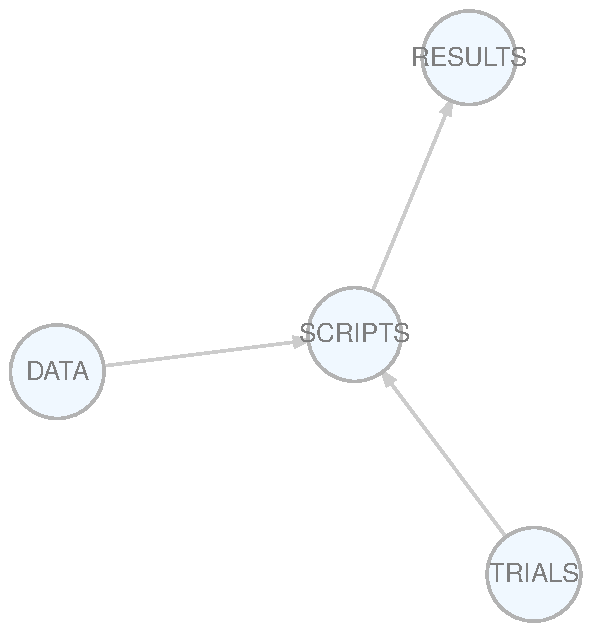
\includegraphics{data/coarse_workflow.pdf}
\caption{Coarse Analytical Workflow\label{Coarse Flow}}
\end{figure}

\newpage

\subsection{\texorpdfstring{Data Acquisition -
\texttt{1\_query\_source.R}}{Data Acquisition - 1\_query\_source.R}}\label{data-acquisition---1_query_source.r}

The objective of the scripts called in
\texttt{scripts/0\_query\_source.R} is to query a data source (such as
Bloomberg, Datastream or iNet) and save the results in an appropriate
format in the \texttt{data/datalog} directory. This directory can grow
without limit. It can be deleted and regenerated from the query scripts.
It will be mined by downstream scripts to create datasets for
backtesting.

\begin{verbatim}
Relevant parts of the directory tree: 

. equity_analysis/
|    data/
|    |   datalog
|    scripts/
|    |   1_query_source.R
|    |   data_processing/
|    |   |   1_bloomberg_to_datalog.R
|    |   |   1_simulated_to_datalog.R
\end{verbatim}

We include two sample scripts. One for querying Bloomberg, the other for
generating simulated dummy data for demonstration purposes. These
scripts can be found in the \texttt{scripts/data\_processing/}
directory. This directory adopts a sequential naming convention because
they are intended to be run sequentially.

\texttt{1\_Bloomberg\_to\_datalog.R} follows the broad procedure of
collecting all the data required to build a dataset. The query script
performs the following steps in a non-interactive manner -

\begin{enumerate}
\def\labelenumi{\arabic{enumi}.}
\tightlist
\item
  Connect to the vendor via an API (in the case of Bloomberg, this is
  via ({\textbf{???}})'s R package Rblpapi).
\item
  Define a target index. For instance, we extract JALSH, which is the
  Johannesburg Securities Exchange (JSE) All Share Index.
\item
  Define how far back to extract constituent lists.
\item
  Extract monthly constituent lists for the index and save to the
  \texttt{datalog}.
\item
  Read in all constituent lists and compile a unique list of tickers.
  These will include delisted shares as well as survivors .
\item
  Define required ticker metadata. At a minimum, the ticker code and the
  ISIN is required. Market data is extracted with the ticker code;
  fundamental data is extracted with the ISIN.
\item
  Extract and save metadata for all tickers.
\item
  Extract and save market data for each tickers based on ticker code.
\item
  Extract and save fundamental data for each tickers based on ISIN.
\end{enumerate}

\subsubsection{File naming conventions}\label{file-naming-conventions}

All queries are saved to the \texttt{data/datalog} directory under the
following naming convention -

\begin{quote}
\texttt{TIMESTAMP\_\_source\_\_data\_type\_\_data\_label}
\end{quote}

Where

\begin{itemize}
\tightlist
\item
  \texttt{TIMESTAMP} is millisecond time, as calculated by
  \texttt{as.numeric(as.POSIXct(Sys.time()))*10\^{}5}.
\item
  \texttt{source} is the data source, such as \texttt{BLOOMBERG}.
\item
  \texttt{data\_type} is one of \texttt{constituent\_list},
  \texttt{metadata\_array}, \texttt{ticker\_fundamental\_data} or
  \texttt{ticker\_market\_data}.
\item
  \texttt{data\_label} is the identifier of the particular object.
\item
  \texttt{constituent\_list} types are of the form
  \texttt{YYYMMDD\_INDEX};
\item
  \texttt{metadata\_array} types are simply the \texttt{INDEX};
\item
  \texttt{ticker\_market\_data} are of the form \texttt{TICKER},
\item
  \texttt{ticker\_fundamental\_data} are of the form \texttt{ISIN}.
\end{itemize}

Using this file naming convention is essential. It allows us to save
many versions of the same data in a manner that is very fast to filter
for downstream processing. Downstream scripts use these filenames to
mine the datalog and build master datasets. An example of a well formed
datalog file name is -

\begin{quote}
\texttt{152874575747280\_\_bloomberg\_\_ticker\_fundamental\_data\_\_ZAE000018131\ Equity.csv}
\end{quote}

\subsubsection{File contents
conventions}\label{file-contents-conventions}

Datalog files should also be Tidy. That is, each file related to a
particular object in the real world (i.e, an index, a metadata array, or
a ticker), and the dat is flat and tablular, with each row being an
observation (i.e a date) and each column an attribute (eg. CLOSE, LOW,
HIGH etc). An example of a Tidy \texttt{fundamental\_data} file is -

\begin{longtable}[]{@{}lrr@{}}
\toprule
date & BS\_ACCT\_NOTE\_RCV & BS\_INVENTORIES\tabularnewline
\midrule
\endhead
2014-12-31 & NA & 1182822\tabularnewline
2015-06-30 & 782550.2 & 1158028\tabularnewline
2015-12-31 & NA & 1260626\tabularnewline
2016-06-30 & 605207.4 & 1048830\tabularnewline
2016-12-31 & NA & 1057549\tabularnewline
2017-06-30 & 522236.0 & 1019666\tabularnewline
\bottomrule
\end{longtable}

\subsubsection{Chunking and reruns}\label{chunking-and-reruns}

It is not necessary that all \texttt{data\_types} attributes are
contained in a single file. For instance, the results of the query to be
saved under filename
\texttt{bloomberg\_\_ticker\_fundamental\_data\_\_ZAE000018131\ Equity.csv}
could be chunked across multiple queries and spread across the files

\begin{quote}
\texttt{152874575747280\_\_bloomberg\_\_ticker\_fundamental\_data\_\_ZAE000018131\ Equity.csv}\\
\texttt{152874575747380\_\_bloomberg\_\_ticker\_fundamental\_data\_\_ZAE000018131\ Equity.csv}\\
\texttt{152874575747480\_\_bloomberg\_\_ticker\_fundamental\_data\_\_ZAE000018131\ Equity.csv}\\
\texttt{152874575747580\_\_bloomberg\_\_ticker\_fundamental\_data\_\_ZAE000018131\ Equity.csv}
\end{quote}

This chunking can be done along either rows or columns or both. Chunking
does not have to be sequential, either. A query can be run multiple
times, saving more and more data to the datalog.

\newpage

\subsection{\texorpdfstring{Data processing -
\texttt{2\_process\_data.R}}{Data processing - 2\_process\_data.R}}\label{data-processing---2_process_data.r}

The \texttt{data/dataset} directory is the canonical data store of the
system. Unstructured data in the datalog is compacted and organised
according to a predictable directory structure inside the dataset
directory.

\begin{verbatim}
Relevant parts of the directory tree: 

. equity_analysis
|    data/
|    |   datalog/
|    |   datasets/
|    |   |  constituent_list/
|    |   |  |  metadata_array.feather
|    |   |  metadata_array/
|    |   |  |  metadata_array.feather
|    |   |  ticker_fundamental_data/
|    |   |  |  ISIN_1.feather
|    |   |  |  ISIN_n.feather
|    |   |  ticker_market_data/
|    |   |  |  ticker_1.feather
|    |   |  |  ticker_n.feather
|    scripts/
|    |   2_process_data.R
|    |   data_processing/
|    |   |   2_datalog_csv_to_feather.R
|    |   |   3_constituents_to_dataset.R
|    |   |   3_metadata_to_dataset.R
|    |   |   3_ticker_logs_to_dataset.R
\end{verbatim}

In order to speed up downstream processing time, all \texttt{.csv} files
in the \texttt{datalog} are converted to \texttt{.feather} format.
\texttt{.feather} files are much faster to read and write, and do not
require the type parsing typically required of \texttt{.csv} files.

The objective of the scripts in \texttt{1\_process\_data.R} is to read
in the contents of the \texttt{datalog}, identify what datasets can be
generated from the logs, and commit them to the \texttt{dataset}
archive. Suitable target datasets are, for instance,
\texttt{metadata/metadata.feather} or
\texttt{ticker\_fundamental\_data/ISIN\_1.feather}.

\subsubsection{Melting}\label{melting}

In contrast to datalogs, datasets are stored in a \emph{tall and narrow}
data structure.

The following table is \emph{short and wide} , with one row per date,
and one column per attribute (note - we omit columns due to limited
space. There are also timestamp and source columns in this table) -

\begin{longtable}[]{@{}lrr@{}}
\toprule
date & BS\_ACCT\_NOTE\_RCV & BS\_INVENTORIES\tabularnewline
\midrule
\endhead
2014-12-31 & NA & 1182822\tabularnewline
2015-06-30 & 782550.2 & 1158028\tabularnewline
2015-12-31 & NA & 1260626\tabularnewline
2016-06-30 & 605207.4 & 1048830\tabularnewline
2016-12-31 & NA & 1057549\tabularnewline
2017-06-30 & 522236.0 & 1019666\tabularnewline
\bottomrule
\end{longtable}

The same table can be converted into \emph{tall and narrow} format using
the \texttt{tidyr:gather()} function into this format -

\begin{longtable}[]{@{}llllr@{}}
\toprule
date & timestamp & source & metric & value\tabularnewline
\midrule
\endhead
2014-12-31 & 152874575747280 & bloomberg & BS\_ACCT\_NOTE\_RCV &
NA\tabularnewline
2015-06-30 & 152874575747280 & bloomberg & BS\_ACCT\_NOTE\_RCV &
782550.2\tabularnewline
2015-12-31 & 152874575747280 & bloomberg & BS\_ACCT\_NOTE\_RCV &
NA\tabularnewline
2016-06-30 & 152874575747280 & bloomberg & BS\_ACCT\_NOTE\_RCV &
605207.4\tabularnewline
2016-12-31 & 152874575747280 & bloomberg & BS\_ACCT\_NOTE\_RCV &
NA\tabularnewline
2017-06-30 & 152874575747280 & bloomberg & BS\_ACCT\_NOTE\_RCV &
522236.0\tabularnewline
2017-12-31 & 152874575747280 & bloomberg & BS\_ACCT\_NOTE\_RCV &
1066796.2\tabularnewline
2014-12-31 & 152874575747280 & bloomberg & BS\_INVENTORIES &
1182822.4\tabularnewline
2015-06-30 & 152874575747280 & bloomberg & BS\_INVENTORIES &
1158028.4\tabularnewline
2015-12-31 & 152874575747280 & bloomberg & BS\_INVENTORIES &
1260625.5\tabularnewline
\bottomrule
\end{longtable}

We do this conversion for a number of reasons. Firstly, it allows us to
filter for a particular data point (i.e, a date, attribute, and ticker
cell) much more quickly by simply filtering each column. This enables
efficient deduplication, compaction and versioning, which reduces the
dataset size dramatically and speeds load, write and procssing
operations.

Secondly, is allows us great flexibility in the attributes we collect.
Collecting variable numbers of attributes in the querying step results
in tables with varying columns. Joining multiple files to create one
dataset on \emph{short and wide} data would require column matching on
every single join operation, which is expensive and error prone. In
contrast, columns are stable when \emph{tall and narrow}. No matter what
the original attributes are, or how they chang across queries, we know
that we will always have the same columns, namely \texttt{date},
\texttt{timestamp}, \texttt{source}, \texttt{metric} and \texttt{value}.

Finally, the \emph{tall and narrow} format allows us to deal with NA
values properly. With this format, we know that if the \texttt{value}
column is \texttt{NA}, then we should drop the row. Consider the
\emph{short and wide} example. There are multiple attributes. Some are
\texttt{NA}, others are not. How do we dealwith this? THere is no easy
way to drop a single attribute for a songle date without dropping the
other attributes for that date. THis is not a big issue for single-query
datalogs. But consider what happens when we have multiple versions of a
datapoint, some of which are \texttt{NA}, and some of which are not.
Finding the latest value of a data point that is not \texttt{NA} and
using that as your latest value is quite complex with \emph{short and
wide} data. For \emph{tall and narrow} data, it's quite simple. Just
filter the rows appropriately, drop any \texttt{NA} entries and then
take the most recent timestamp. Dropping of \texttt{NA} values is done
without loss of information, since recasting into \emph{short and
narrow} format inserts \texttt{NA} values into empty cells.

\emph{Tall and wide} formats also have disadvantages, especially when
one wants to perform rowwise computations across attributes. Because of
this, we convert the datasets back to \emph{short and narrow} format
during backtesting.

\subsubsection{Using dataframes rather than timeseries
objects}\label{using-dataframes-rather-than-timeseries-objects}

R supports several timeseries data structures, including \texttt{ts},
\texttt{zoo} and \texttt{xts} formats. These formats come with methods
that are very useful for the manipulation of time series. We have
decided to use dataframes instead of these formats because they require
that all attributes be the same data type. This is a consequence of the
fact that the \texttt{zoo} package is actually an indexed matrix;
matrices in R can only be one data type. Sticking with dataframes allows
us to mix many types of data in our timeseries.

\subsubsection{Script procedures}\label{script-procedures}

The series of scripts sourced in \texttt{1\_process\_data.R} each
perform the following procedures -

\begin{enumerate}
\def\labelenumi{\arabic{enumi}.}
\tightlist
\item
  Read all files in the \texttt{datalog} into a dataframe, splitting
  each fieldname into an appropriate column.
\item
  From the file names, determine the set of datasets that can be
  generated from the logfiles.
\item
  For each dataset:

  \begin{itemize}
  \tightlist
  \item
    Read in logfiles relevant to the dataset
  \item
    Convert to \emph{tall and narrow} format
  \item
    Check if a dataset already exists and, if it does, read it in to
    memory
  \item
    Join the datasets
  \item
    Filter out and NA values
  \item
    Remove any duplicates
  \item
    Filter out any records that have not changed since the last
    timestamp, but update the timestamp field
  \end{itemize}
\end{enumerate}

The end result is a set of directories in \texttt{data/datasets}.
Because the scripts merge, rather than overwrite datset files it is
possible (but not necessary) to periodically empty or delete the datalog
wothout loss of information.

The files in the the \texttt{datasets} directories are \textbf{not}
Tidy. In particular -

\begin{enumerate}
\def\labelenumi{\arabic{enumi}.}
\tightlist
\item
  Each file does not correspond real thing. The constituent and metadata
  files contain all data for all indexes and tickers in a single file.
\item
  Each attribute is not a column.
\end{enumerate}

The datsets are converted to Tidy format in-memory at backtest runtime.

\newpage

\subsection{\texorpdfstring{Backtesting -
\texttt{3\_run\_trials.R}}{Backtesting - 3\_run\_trials.R}}\label{backtesting---3_run_trials.r}

Unlike the data processing scripts, the backtesting scripts are not
named in a sequential fashion. This is because their sourcing is not
sequential.

\begin{verbatim}
Relevant parts of the directory tree: 

. equity_analysis/
|    data/
|    |   datasets/
|    scripts/
|    |   3_run_trials.R
|    |   trading/
|    |   |   example_trial.R
|    |   |   load_slow_moding_data.R
|    |   |   trade.R
|    trials/
|    results/
\end{verbatim}

Rather, these scripts follow a parent - child relationship. The parent
script is \texttt{3\_run\_trials.R}. It sources the other scripts and
uses their functions when necessary. Understanding how backtesting is
accomplished is best achieved by working through this script from top to
bottom, referring to other scripts when they are called.

\subsubsection{Global parameters}\label{global-parameters}

The first section of the script sets parameters global to the session.
These parameters are -

\begin{enumerate}
\def\labelenumi{\arabic{enumi}.}
\tightlist
\item
  Mode

  \begin{itemize}
  \tightlist
  \item
    \texttt{run\_mode} - BACKTEST or LIVE. LIVE mode not yet
    implemented.
  \item
    \texttt{heartbeat\_duration} - time between trade loops, in seconds.
    Typically between 600 and 3600.
  \end{itemize}
\item
  Universe

  \begin{itemize}
  \tightlist
  \item
    \texttt{constituent\_index} - index to backtest against.
  \item
    \texttt{data\_source} - data source to use.
  \item
    \texttt{market\_metrics} - market metrics to filter (defaults to
    all).
  \item
    \texttt{fundamental\_metrics} - fundamental metrics to filter
    (defaults to all).
  \end{itemize}
\item
  Timeframe

  \begin{itemize}
  \tightlist
  \item
    \texttt{start\_backtest} - YYYYMMDD start of backtest.
  \item
    \texttt{end\_backtest} - YYYYMMDD end of backtest.
  \end{itemize}
\item
  Portfolio Characteristics

  \begin{itemize}
  \tightlist
  \item
    \texttt{portfolio\_starting\_config} - CASH or STOCK. CASH
    initialises the portfolio with 100\% cash. STOCK initialises the
    portfolio with perfect portfolio weights at start. STOCK not
    implemented yet.
  \item
    \texttt{portfolio\_starting\_value} - starting cash value of
    portfolio.
  \item
    \texttt{cash\_buffer\_percentage} - desired cash percentage of
    portfolio to target.
  \end{itemize}
\item
  Trading characteristics

  \begin{itemize}
  \tightlist
  \item
    \texttt{commission\_rate} - percentage of trade value charged as
    commission.
  \item
    \texttt{minimum\_commission} - minimum value of commission.
  \item
    \texttt{standard\_spread} - simple assumed spread between bid and
    ask, expressed as a percentage of stock price.
  \end{itemize}
\end{enumerate}

We see from these parameters that the backtester uses a stock index as
the defining unit of a stock universe. It can only use one data source
at a time, but synthetic datasets can be build in the data pipeline
stage. It expects a start and end date for the backtest, and we have to
specify a portfolio starting value and desired cash buffer. This is
because excess returns are portfolio seize dependent. Large portfolios
may not be able to trade illiquid stocks; small portfolios may suffer
from high commissions. We have also specified rudimentary transaction
cost modeling and slippage, in the form of a simple commission structure
and a standard spread which will be imposed at trade.

The script runs \texttt{trade.R} against each \texttt{algorithm\_X.R}
file in the \texttt{trials/} directory, saving the results, and the
\texttt{algorithm\_X.R} file, to its own subdirectory in the
\texttt{results/} directory. The subdirectory naming convention is
\texttt{INDEX\_\_algorithmX}.

That is, an algorthm named \texttt{market\_weighted.R}, run against the
index \texttt{JALSH} will result in a results subdirectory
\texttt{JALSH\_\_market\_weighted}. This subdirectory will contain the
original \texttt{market\_weighted.R} file as well as several reporting
and runtime history files. It is therefore possible to take a
\texttt{results} subdirectory contents, rerun the algorithm, and compare
with the original results.

{[}FLOW CHART OF OPERATIONS INSIDE THE TRADE SECTION{]}

\subsubsection{\texorpdfstring{The \texttt{ticker\_data} and
\texttt{runtime\_ticker\_data}
objects}{The ticker\_data and runtime\_ticker\_data objects}}\label{the-ticker_data-and-runtime_ticker_data-objects}

The trading engine reuses several dataframes during the course of
operation. Two of these are critical to understanding how it avoids
look-ahead bias and generates trades.

\begin{enumerate}
\def\labelenumi{\arabic{enumi}.}
\tightlist
\item
  The \texttt{ticker\_data} data object is a list of dataframes
  containing tickers relevant to the backtest. It is \textbf{not} free
  of survivorship bias or look ahead bias. It is constructed by sourcing
  \texttt{load\_slow\_moving\_data.R}, which expects to find
  \texttt{3\_run\_trials.R} parameters in the global environment.

  \begin{enumerate}
  \def\labelenumii{\arabic{enumii}.}
  \tightlist
  \item
    It reads in the \texttt{constituent.feather} and
    \texttt{metadata.feather} datasets, and filters these datasets to
    include only \texttt{source} and \texttt{index} parameters included
    in the global environment.
  \item
    It then constructs a list of dataframes, where each dataframe
    contains the market and fundamental data of a ticker in the filtered
    constituent list, joined on the metadata market and fundamental
    identifier fields.
  \item
    It filters all dataframes to take only the most recent timestamp
    version of data points with multiple timestamped versions.
  \item
    It spreads the dataframes into \emph{short and wide}, Tidty form.
  \end{enumerate}
\item
  The \texttt{runtime\_ticker\_data} data object is derived from
  \texttt{ticker\_data} and \textbf{is} free of survivorship and
  look-ahead bias. It is recomputed every time the
  \texttt{runtime\_date} (i.e the date that the trading engine
  \emph{thinks} it is) changes, and is computed by calling the
  \texttt{get\_runtime\_dataset} function. This function takes
  \texttt{execution\_date}, \texttt{constituent\_list} and
  \texttt{ticker\_data} objects as arguments, and returns a subset of
  \texttt{ticker\_data} that contains only those constituents that were
  in the constituent list at the execution date, and only those data
  points that were available prior to the execution date. It also
  backfills any \texttt{NA} values with the last known value. This
  converts low-periodicity data, such as balance sheet line items, into
  daily data for easy row-wise operations.
\end{enumerate}

\subsubsection{\texorpdfstring{The \texttt{compute\_weights}
function}{The compute\_weights function}}\label{the-compute_weights-function}

This function comprises the entire contents of a
\texttt{trials/algorithm\_X.R} script. This function is designed by the
researcher, and must take in an in-memory \texttt{runtime\_ticker\_data}
dataset and a vector of \texttt{metrics}(ticker attributes), and returns
a list of ideal portfolio weights. That is, it reads in the state of the
world as it would appear at \texttt{runtime\_date} and makes some
decision about what the optimal portfolio weighting should be. This
decision rule can be whatever the researcher wants, and can make full
use of the R universe of statistical packages in construction.

The power of this arrangement is that it allows a researcher to modify
the weighting algorithm while holding all other variables constant.
Because it accepts a whole \texttt{runtime\_ticker\_data} object, it can
conduct \texttt{map} operations across the entire list fo dataframes -
it can specify the target weight of a ticker contingent on, say, its
ranking amongst all other tickers based on some ranking procedure that
accepts arbitrary attributes. This is immensely flexible - one can build
\texttt{map} operations that set all non-industrial stocks to weight 0,
for instance, or nest rankings according to sector and then hard-code
overall sector weights.

Because the wrapper script \texttt{trade.R} only cares about getting
back a vector with portfolio weights, the internals of the function can
be very elaborate. It would be entirely possible to spin up an
\texttt{h2o} machine learning instance inside this function, train a
deep learning model, predict an outcome and use that classification to
return \texttt{target\_weights}. Because we know that the function only
has access to bias-free data, we know the predictions wont be able to
cheat. Since the dataframes are in Tidy format, they are accepted
without modification by many R model-fitting packages.

Since these weights only need to be recomputed daily, this training can
take quite long. Higher frequency prediction would constrain model
complexity to occur within the heartbeat window.

\subsubsection{Trade submission
procedure}\label{trade-submission-procedure}

The \texttt{trade.R} script performs the following operations -

\begin{enumerate}
\def\labelenumi{\arabic{enumi}.}
\tightlist
\item
  Source the \texttt{algorithm.R} script.
\item
  Set \texttt{heartbeat\_count} to 0.
\item
  Set \texttt{runtime\_date} to start of backtest +
  \texttt{heartbeat\_count}.
\item
  Check if \texttt{ticker\_data} has been loaded to memory and if it is
  less than 24 hours (in heartbeat time) old.

  \begin{itemize}
  \tightlist
  \item
    If not, reload \texttt{ticker\_data} by sourcing
    \texttt{load\_slow\_moving\_data.R}
  \end{itemize}
\item
  Check if \texttt{runtime\_ticker\_data} is less than 24 hours (in
  heartbeat time) old.

  \begin{itemize}
  \tightlist
  \item
    If not, run \texttt{get\_runtime\_dataset} again and then run
    \texttt{compute\_weights} again to obtain new
    \texttt{target\_weights}. We only re-compute
    \texttt{target\_weights} when \texttt{runtime\_ticker\_data} changes
    because it is the only input to the \texttt{compute\_weights}
    function.
  \end{itemize}
\item
  Get the \texttt{transaction\_log} and \texttt{trade\_history} data
  objects and compute our current portfolio and cash positions.
\item
  Query latest prices for the positons to obtain a portfolio valuation.
\item
  Compute \texttt{trades} by calling \texttt{compute\_trades}, using
  \texttt{target\_weights} and \texttt{positions} as arguments.
\item
  Submit \texttt{trades} by calling the \texttt{submit\_orders}
  function, using \texttt{trades} as an argument.
\item
  Increment the \texttt{heartbeat\_count} value by the global
  \texttt{hearbeat\_duration} value.
\item
  Repeat steps 3 - 10 until \texttt{runtime\_date} is equal to or
  greater than \texttt{end\_backtest}.
\end{enumerate}

In a live environment, the \texttt{submit\_trades()} function would
submit the trades to a broker via the broker-supplied API. Submitted
trades would be matched (or partially matched) by an external broker and
our broker-side trade history and transaction logs would be updated. In
this setup, getting \texttt{transaction\_log} and
\texttt{trade\_history} objects would amount to querying the broker API
and saving the result to the \texttt{results/INDEX\_\_algorithmX}
subdirectory. These logs are avaiable to the trade loop and perform the
function of updating the portfolio weights, allowing a new
\texttt{trades} object to be computed.

In a backtest environment, this trade matching needs to be simulated. In
this context, the \texttt{submit\_orders()} function simulates the
actions of an extenral broker. This function accepts a \texttt{trades}
dataframe as an argument, and then -

\begin{enumerate}
\def\labelenumi{\arabic{enumi}.}
\tightlist
\item
  Obtains price quotes for each ticker in the \texttt{trades} dataframe.
  The \texttt{get\_stock\_quote} function queries ticker\_data for the
  highest price, lowest price and volume on the execution date, and then
  selects a random sample of size 1 for the price range. This random
  sample is the \texttt{midpoint}. The \texttt{bid} and \texttt{offer}
  are computed as the difference of \texttt{midpoint} and the
  \texttt{spread}, as defined in the global parameters. It then computes
  the \texttt{size} of available units as daily volume divided by
  (trading day / heartbeat duration). That is, it assigns trading lots
  uniformly thoughout the day. In this manner, liquidity is constrained
  to a reasonable approximation of the volume that would have been
  available throughout the day. Finally, it returns a vector with the
  \texttt{bid}, \texttt{ask} and \texttt{size}.
\item
  Computes successful trades as those where the correct side (i.e bid
  for a sell order, ask for a buy order) is within the limit order price
  specified in the \texttt{trades} dataframe.
\item
  Assigns a trade size (the minimum of units avaialble and units asked
  for) to each trade.
\item
  Generates a session trade log and transaction history
\item
  Reads in the \texttt{trade\_history} and \texttt{transaction\_log}
  objects.
\item
  Appends the session values
\item
  Saves the \texttt{trade\_history} and \texttt{transaction\_log}
  objects to file
\item
  Returns a short summary of successful trades.
\end{enumerate}

\subsubsection{Backtest results}\label{backtest-results}

A well specified \texttt{compute\_weights} function will result in a
successful backtest. The results of each backtest run by
\texttt{3\_run\_trials.R} will be placed in the \texttt{results}
directory according to the naming convention covered earlier.

These \texttt{results} subdirectories contain five files -

\begin{enumerate}
\def\labelenumi{\arabic{enumi}.}
\tightlist
\item
  The original \texttt{algorithm\_X.R} script from the \texttt{trials}
  directory.
\item
  A \texttt{runtime\_log} file, which contains relevant runtime
  information. Each line of this file represents another heartbeat.
\item
  A \texttt{trade\_history.feather} file, which contains a full trade
  history, similar to what would be obtained from an external broker.
\item
  A \texttt{transaction\_log.feather} file, which contains a full
  transaction log, similar to what would be obtained fro an external
  broker. This log is analogous to a bank account, and keeps track of
  account cash balances as trades, deposits, withdrawals and account
  charges are levied.
\item
  A \texttt{summary\_statistics.Rmd} file, which presents an historical
  summary of the strategy performance, including (but not limited to)
  sharpe ratio, annualized return over a range of horizons, maximum
  drawdown, turnover and total expense ratio.
\end{enumerate}

\newpage

\subsection{Cross Validation}\label{cross-validation}

\newpage

\subsection{Reporting}\label{reporting}

Must address:

\begin{enumerate}
\def\labelenumi{\arabic{enumi}.}
\item
  Survivorship bias
\item
  Look ahead bias
\item
  Completeness: multi source
\item
  Retroactive corrections: dataset monitoring
\item
  Market impact
\item
  Transaction Costs
\item
  Portfolio bankruptcy
\item
  Backtest overfitting: pbo
\end{enumerate}

Must try to:

\begin{enumerate}
\def\labelenumi{\arabic{enumi}.}
\tightlist
\item
  Be convertalbe to live with minimal effort
\item
  Acommodate any sort of date
\item
  Be interoperable with other packages (xes\ldots{})
\item
  Use tidy data structures
\end{enumerate}

Second-order challenges Compaction: dropping useless data Speed:
training vs trading Speed: parallel processing Speed: read/write:
feather Memory: filtering and subsetting

\subsection{Features}\label{features}

\begin{itemize}
\tightlist
\item
  data versioning
\item
  multi-source
\item
  multi-index
\item
  code version control
\item
  clear procedural workflow
\item
  event-driven
\item
  tidy data
\item
  pbo
\item
  host of metrics
\item
  bias avoidance
\end{itemize}

\section{\texorpdfstring{Conclusion\label{conclusion}}{Conclusion}}\label{conclusion}

This paper has explored the various ways in which the lack of
transparency in anomalies research makes it difficult to discern
spurious results from geniune findings. This `replication crisis' has
strong analogues in other academic disciplines. We have argued that the
`reproducible science' response to this crisis in science at large has
potential to address much of the issues that bedevil anomalies
replication.

We have introduced a collection of R scripts, organised into a
compendium, that can be used to conduct anomalies research in a
transparent and reproducible way. These scripts utilize only free, open
source software and to organize data along the lines of `tidy' data.
Using plain text computer code to collect, process, structure and
analyse data represents a good approach to producing research that is
easy to reproduce.

We avoid the problem of proprietary data distribution by including
customizable data query scripts. These scripts query proprietary vendors
and save the results in a standard way. Bundling these query scripts in
a compendium enables a replicator to rebuild the dataset programatically
and non-interactively from source.

This collection of scripts make it possible to test an investment
algorithm against an index of stocks, where each stock comprises a set
of daily observations of price data plus an arbitrary number of
attributes. The scripts use the event-based backtest method (as opposed
to vectorized methods) which make it easy to avoid look-ahead bias and
to introduce non-standard data to the algorithm. Transaction cost and
slippage modelling, while rudimentary, exist and can be refined.

Using this code base as a starting point should save a research a great
deal of time in preparing stock data for backtesting, and the open
source nature of the project ensures that any researcher can comb the
operations for bugs or implement features that are not present. While it
is not expected that this code base is necessary or sufficient for
end-to-end backtesting, it represents a solid base for ongoing
development.

Katzke (\protect\hyperlink{ref-Katzke2017}{2017})

\section*{References}\label{references}
\addcontentsline{toc}{section}{References}

\hypertarget{refs}{}
\hypertarget{ref-Bache2014}{}
Bache, Stefan Milton, and Hadley Wickham. 2014. ``magrittr: A
Forward-Pipe Operator for R.''
\url{https://cran.r-project.org/package=magrittr}.

\hypertarget{ref-Bailey2014}{}
Bailey, David H., Jonathan M. Borwein, Marcos López de Prado, and Qiji
Jim Zhu. 2014. ``Pseudo-Mathematics and Financial Charlatanism: The
Effects of Backtest Overfitting on Out-of-Sample Performance.''
\emph{Notices of the AMS} 61 (5): 458--71.
doi:\href{https://doi.org/10.2139/ssrn.2308659}{10.2139/ssrn.2308659}.

\hypertarget{ref-Baum2002}{}
Baum, Christopher F., and Selcuk Sirin. 2002. ``Why should you avoid
using point-and-click method in statistical software packages?''
\url{http://fmwww.bc.edu/GStat/docs/pointclick.html}.

\hypertarget{ref-Baumer2014}{}
Baumer, Ben, Mine Cetinkaya-Rundel, Andrew Bray, Linda Loi, and Nicholas
J. Horton. 2014. ``R Markdown: Integrating A Reproducible Analysis Tool
into Introductory Statistics.''
doi:\href{https://doi.org/10.5811/westjem.2011.5.6700}{10.5811/westjem.2011.5.6700}.

\hypertarget{ref-Carl2018}{}
Carl, Peter, Brian G Peterson, Joshua Ulrich, and Jan Humme. 2018.
\emph{quantstrat: Quantitative Strategy Model Framework}.

\hypertarget{ref-Damodaran2012}{}
Damodaran, A. 2012. \emph{Investment Philosophies: Successful Strategies
and the Investors Who Made Them Work}. Wiley Finance Editions. Wiley.
\url{https://books.google.co.za/books?id=NkOkN0l3vHgC}.

\hypertarget{ref-Fama1992}{}
Fama, E., and K. French. 1992. ``The Cross-Section of Expected Stock
Returns.'' doi:\href{https://doi.org/10.2307/2329112}{10.2307/2329112}.

\hypertarget{ref-Gentleman2004}{}
Gentleman, Robert, and Duncan Lang. 2004. ``Statistical Analyses and
Reproducible Research.''

\hypertarget{ref-Graham1934a}{}
Graham, B, D Dodd, and D L F Dodd. 1934. \emph{Security Analysis: The
Classic 1934 Edition}. McGraw-Hill Education.
\url{https://books.google.co.za/books?id=wXlrnZ1uqK0C}.

\hypertarget{ref-Hou2017}{}
Hou, Kewei, Chen Xue, and Lu Zhang. 2017. ``Replicating anomalies.''
\emph{NBER Working Papers}, no. No. 23394.
doi:\href{https://doi.org/10.2139/ssrn.2190976}{10.2139/ssrn.2190976}.

\hypertarget{ref-Ioannidis2005}{}
Ioannidis, John P. A. 2005. ``Why Most Published Research Findings Are
False.'' \emph{PLoS Medicine} 2 (8). Public Library of Science: e124.
doi:\href{https://doi.org/10.1371/journal.pmed.0020124}{10.1371/journal.pmed.0020124}.

\hypertarget{ref-Katzke2017}{}
Katzke, N F. 2017. ``Texevier: Package to create Elsevier templates for
Rmarkdown.'' Stellenbosch, South Africa.

\hypertarget{ref-Koenker2009}{}
Koenker, Roger, and Achim Zeileis. 2009. ``On reproducible econometric
research.'' \emph{Journal of Applied Econometrics}.
doi:\href{https://doi.org/10.1002/jae.1083}{10.1002/jae.1083}.

\hypertarget{ref-Li2004}{}
Li, Shengying. 2004. ``A Survey on Tools for Binary Code Analysis.''

\hypertarget{ref-LopezdePrado2013}{}
Lopez de Prado, Marcos. 2013. ``The Probability of Back-Test
Over-Fitting.'' \emph{SSRN Electronic Journal}.
doi:\href{https://doi.org/10.2139/ssrn.2308682}{10.2139/ssrn.2308682}.

\hypertarget{ref-Marwick2018}{}
Marwick, Ben, Carl Boettiger, and Lincoln Mullen. 2018. ``Packaging Data
Analytical Work Reproducibly Using R (and Friends).'' \emph{American
Statistician}.
doi:\href{https://doi.org/10.1080/00031305.2017.1375986}{10.1080/00031305.2017.1375986}.

\hypertarget{ref-Munafo2017}{}
Munafò, Marcus R, Brian A Nosek, Dorothy V.M. Bishop, Katherine S
Button, Christopher D Chambers, Nathalie Percie Du Sert, Uri Simonsohn,
Eric Jan Wagenmakers, Jennifer J Ware, and John P.A. Ioannidis. 2017.
``A manifesto for reproducible science.''
doi:\href{https://doi.org/10.1038/s41562-016-0021}{10.1038/s41562-016-0021}.

\hypertarget{ref-Peterson2017}{}
Peterson, Brian G. 2017. ``Developing \& Backtesting Systematic Trading
Strategies,'' no. June: 42.
doi:\href{https://doi.org/10.20964/2016.12.40}{10.20964/2016.12.40}.

\hypertarget{ref-Quantopian2018}{}
Quantopian. 2018. ``Improved Backtest Analysis.''
\url{https://www.quantopian.com/posts/improved-backtest-analysis}.

\hypertarget{ref-Quantpedia2018}{}
Quantpedia. 2018. ``Backtesting Software.''
\url{https://quantpedia.com/Links/Backtesters}.

\hypertarget{ref-RCoreTeam2018}{}
R Core Team. 2018. ``R: A Language and Environment for Statistical
Computing.'' Vienna, Austria. \url{https://www.r-project.org/}.

\hypertarget{ref-Raymond:2003:AUP:829549}{}
Raymond, Eric S. 2003. \emph{The Art of UNIX Programming}. Pearson
Education.

\hypertarget{ref-RStudioTeam2015}{}
RStudio Team. 2015. ``RStudio: Integrated Development Environment for
R.'' Boston, MA. \url{http://www.rstudio.com/}.

\hypertarget{ref-Stodden2013}{}
Stodden, V, D H Bailey, J Borwein, R J Leveque, W Rider, and W Stein.
2013. ``Setting the Default to Reproducible Reproducibility in
Computational and Experimental Mathematics.'' In \emph{ICERM Workshop},
19. \url{http://www.davidhbailey.com/dhbpapers/icerm-report.pdf}.

\hypertarget{ref-Trice2017}{}
Trice, Tim. 2017. \emph{Backtesting Strategies with R}.
\url{https://timtrice.github.io/backtesting-strategies/index.html}.

\hypertarget{ref-VanRoy2009}{}
Van Roy, P. 2009. ``Programming Paradigms for Dummies: What Every
Programmer Should Know.'' \emph{New Computational Paradigms for Computer
Music}, 9--47.
doi:\href{https://doi.org/10.1016/j.tet.2003.02.005}{10.1016/j.tet.2003.02.005}.

\hypertarget{ref-Wickham2014}{}
Wickham, Hadley. 2014. ``Tidy Data.'' \emph{Journal of Statistical
Software}.
doi:\href{https://doi.org/10.18637/jss.v059.i10}{10.18637/jss.v059.i10}.

\hypertarget{ref-Wickham2017}{}
---------. 2017. ``tidyverse: Easily Install and Load the 'Tidyverse'.''
\url{https://cran.r-project.org/package=tidyverse}.

\hypertarget{ref-Zipline2018}{}
Zipline. 2018. ``Zipline Beginner Tutorial --- Zipline 1.3.0
documentation.'' \url{https://www.zipline.io/beginner-tutorial.html}.

% Force include bibliography in my chosen format:

\bibliographystyle{Tex/Texevier}
\bibliography{Tex/ref}





\end{document}
